% ------------------------------------------------------------------------------
% TYPO3 CMS 8.4 - What's New - Chapter "Deprecated Functions" (Spanish Version)
%
% @author	Michael Schams <schams.net>
% @license	Creative Commons BY-NC-SA 3.0
% @link		http://typo3.org/download/release-notes/whats-new/
% @language	English
% ------------------------------------------------------------------------------
% LTXE-CHAPTER-UID:		3f842373-9262b8d3-f9c8de76-cf29ce17
% LTXE-CHAPTER-NAME:	Deprecated Functions
% ------------------------------------------------------------------------------

\section{Funciones Obsoletas/Eliminadas}
\begin{frame}[fragile]
	\frametitle{Funciones Obsoletas/Eliminadas}

	\begin{center}\huge{Capítulo 5:}\end{center}
	\begin{center}\huge{\color{typo3darkgrey}\textbf{Funciones Obsoletas/Eliminadas}}\end{center}

\end{frame}

% ------------------------------------------------------------------------------
% LTXE-SLIDE-START
% LTXE-SLIDE-UID:		04bd9c88-5c86a275-4d264b21-8f0c9902
% LTXE-SLIDE-ORIGIN:	cf7400eb-0f683329-f6c51cbf-dfd192d9 English
% LTXE-SLIDE-TITLE:		#77630: Remove wizard icons
% ------------------------------------------------------------------------------
\begin{frame}[fragile]
	\frametitle{Funciones Obsoletas/Eliminadas}
	\framesubtitle{Iconos del Asistente Eliminados}

	\begin{itemize}

		\item Se han eliminado los siguientes iconos del FormFieldWizard:

			\begin{itemize}
				\item \texttt{wizard\_add.gif}
				\item \texttt{wizard\_edit.gif}
				\item \texttt{wizard\_link.gif}
				\item \texttt{wizard\_list.gif}
				\item \texttt{wizard\_rte.gif}
				\item \texttt{wizard\_table.gif}
			\end{itemize}

	\end{itemize}

	\begin{figure}
		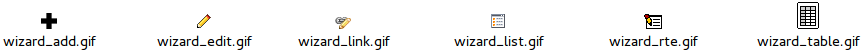
\includegraphics[width=0.95\linewidth]{DeprecatedRemovedFunctions/77630.png}
	\end{figure}

\end{frame}

% ------------------------------------------------------------------------------
% LTXE-SLIDE-START
% LTXE-SLIDE-UID:		5ab1cac5-a53c8f8a-ba56f2a7-c58fa5d5
% LTXE-SLIDE-ORIGIN:	d5ced5e7-04dffe16-b8ec9f2c-712020cd English
% LTXE-SLIDE-TITLE:		#77693: Remove/Move Icons from EXT:t3skin
% ------------------------------------------------------------------------------

\begin{frame}[fragile]
	\frametitle{Funciones Obsoletas/Eliminadas}
	\framesubtitle{Iconos de \texttt{EXT:t3skin}}

	\begin{itemize}

		\item Los iconos de \texttt{EXT:t3skin} han sido eliminados o movidos
		\item \textbf{Eliminados:}

			\begin{itemize}
				\item \smaller\texttt{typo3/sysext/t3skin/icons/gfx/error.png}
				\item \texttt{typo3/sysext/t3skin/icons/gfx/i/\_icon\_ftp.gif}
				\item \texttt{typo3/sysext/t3skin/icons/gfx/information.png}
				\item \texttt{typo3/sysext/t3skin/icons/gfx/notice.png}
				\item \texttt{typo3/sysext/t3skin/icons/gfx/warning.png}
			\end{itemize}

		\item \textbf{Movidos:}

			\begin{itemize}
				\item \smaller\texttt{typo3/sysext/t3skin/icons/gfx/icon\_fatalerror.gif}
				\item \texttt{typo3/sysext/t3skin/images/icons/status/status-edit-read-only.png}
				\item \texttt{typo3/sysext/t3skin/images/icons/status/warning-in-use.png}
				\item \texttt{typo3/sysext/t3skin/images/icons/status/warning-lock.png}
				\item \texttt{typo3/sysext/t3skin/images/icons/status/status-reference-hard.png}
				\item \texttt{typo3/sysext/t3skin/images/icons/status/status-reference-soft.png}
			\end{itemize}

	\end{itemize}

\end{frame}

% ------------------------------------------------------------------------------
% LTXE-SLIDE-START
% LTXE-SLIDE-UID:		8fffd225-8d42b0eb-ae84aa03-680849bf
% LTXE-SLIDE-ORIGIN:	7848f0b0-d687b337-f7638646-680dc819 English
% LTXE-SLIDE-TITLE:		Obsolete page tree and click menu settings removed
% ------------------------------------------------------------------------------

\begin{frame}[fragile]
	\frametitle{Funciones Obsoletas/Eliminadas}
	\framesubtitle{Ajustes del árbol de páginas y del menú de clics}

	\begin{itemize}

		\item Se han eliminado los ajustes obsoletos del árbol de páginas y del menú de clics
		\item \textbf{Propiedades}:

		\begin{itemize}
			\item \texttt{FileSystemNavigationFrameController->doHighlight}
			\item \texttt{ClickMenu->leftIcons}
		\end{itemize}

		\item \textbf{Ajustes TypoScript}:

		\begin{itemize}
			\item \texttt{options.pageTree.disableTitleHighlight}
			\item \texttt{options.contextMenu.options.leftIcons}
		\end{itemize}

	\end{itemize}

\end{frame}

% ------------------------------------------------------------------------------
% LTXE-SLIDE-START
% LTXE-SLIDE-UID:		cc696d46-66e8f8d3-22e98699-04852411
% LTXE-SLIDE-ORIGIN:	aad23a73-7b046eaf-fb4bb862-2f88ef71 English
% LTXE-SLIDE-TITLE:		ExtensionManagementUtility::extRelPath()
% LTXE-SLIDE-REFERENCE:	#78193: ExtensionManagementUtility::extRelPath() deprecated
% ------------------------------------------------------------------------------

\begin{frame}[fragile]
	\frametitle{Funciones Obsoletas/Eliminadas}
	\framesubtitle{ExtensionManagementUtility::extRelPath()}

	\begin{itemize}

		\item Método \texttt{ExtensionManagementUtility::extRelPath()} ha sido declarado obsoleto
		\item Este método se utilizó para resolver rutas relativas al script actual
		\item Están disponibles estos métodos alternativos:
			\begin{itemize}
				\item \texttt{ExtensionManagementUtility::extPath()}\newline
					(para resolver la ruta completa de una extensión)
				\item \texttt{ExtensionManagementUtility::siteRelPath()}\newline
					(para resolver la ubicación de una extensión relativa a \texttt{PATH\_site})
				\item \texttt{GeneralUtility::getFileAbsFileName()}\newline
					(para resolver un fichero/ruta prefijado con EXT:myextension)
				\item \texttt{PathUtility::getAbsoluteWebPath()}\newline
					(para sacar una ubicación de un fichero que tiene un prefijo absoluto para la carpeta web)
			\end{itemize}

	\end{itemize}

\end{frame}

% ------------------------------------------------------------------------------
% LTXE-SLIDE-START
% LTXE-SLIDE-UID:		5a0a58b7-f399bb4c-6940c497-b4375ba5
% LTXE-SLIDE-ORIGIN:	43a5eaf5-8945a8d5-ac27d4ea-24ffc8e3 English
% LTXE-SLIDE-TITLE:		Miscellaneous (1) (#75363)
% LTXE-SLIDE-REFERENCE:	#75363: Deprecate FormResultCompiler->JStop()
% LTXE-SLIDE-REFERENCE:	#75637: Deprecate optional parameters of RecyclerUtility::getRecordPath()
% ------------------------------------------------------------------------------

\begin{frame}[fragile]
	\frametitle{Funciones Obsoletas/Eliminadas}
	\framesubtitle{Miscelánea (1)}

	\begin{itemize}
		\item Método \texttt{FormResultCompiler->JStop()} ha sido renombrado a \texttt{addCssFiles()}.
			El nombre del método antiguo sigue presente como un alias obsoleto, que se eliminará en TYPO3 v9.

		\item Método \texttt{ClickMenu::DB\_editPageProperties()} ha sido declarado obsoleto

		\item Los siguientes argumentos de método \texttt{RecyclerUtility::getRecordPath()} han sido declarados obsoletos:

			\begin{itemize}
				\item \texttt{\$clause}
				\item \texttt{\$titleLimit}
				\item \texttt{\$fullTitleLimit}
			\end{itemize}

	\end{itemize}

\end{frame}

% ------------------------------------------------------------------------------
% LTXE-SLIDE-START
% LTXE-SLIDE-UID:		2dda39d1-c79a756a-24730c12-a44929c0
% LTXE-SLIDE-ORIGIN:	0745e3f3-83db03d7-ac24e92a-300391ba English
% LTXE-SLIDE-TITLE:		Miscellaneous (2) (#77783 and #77826)
% LTXE-SLIDE-REFERENCE:	#77783: Unused ExtJS JavaScript libraries removed
% LTXE-SLIDE-REFERENCE:	#77826: RTEHtmlArea Spellchecker eID removed
% ------------------------------------------------------------------------------

\begin{frame}[fragile]
	\frametitle{Funciones Obsoletas/Eliminadas}
	\framesubtitle{Miscelánea (2)}

	\begin{itemize}

		\item Se han eliminado las siguientes bibliotecas JavaScript ExtJS no utilizadas:

			\begin{itemize}
				\item \texttt{app.SearchField}
				\item \texttt{grid.RowExpander}
				\item \texttt{ux.FitToParent}
			\end{itemize}

		\item RTEHtmlArea eID (\texttt{rtehtmlarea\_spellchecker}) para usar la comprobación ortográfica dinámica ha sido eliminado y el punto de entrada para solicitudes HTTP
			\texttt{SpellCheckingController->main} ha sido declarado obsoleto

		\item Formato \texttt{DateTime::ISO8601} es incompatible con ISO-8601,
			pero se deja por razones de compatibilidad hacia atrás.
			Se utiliza la constante \texttt{DateTime::ATOM} o \texttt{DATE\_ATOM} en su lugar.

	\end{itemize}

\end{frame}

% ------------------------------------------------------------------------------
% LTXE-SLIDE-START
% LTXE-SLIDE-UID:		626ffd35-8f1361d7-e9507c13-52fcaed5
% LTXE-SLIDE-ORIGIN:	0745e3f3-83db03d7-ac24e92a-300391ba English
% LTXE-SLIDE-TITLE:		Miscellaneous (3) (#77839, #78096 and #78222)
% LTXE-SLIDE-REFERENCE:	#77839: TYPO3/CMS/Core/QueryGenerator
% LTXE-SLIDE-REFERENCE:	#78096: Deprecate PageLayoutView::getResult with mysqli_result objects
% LTXE-SLIDE-REFERENCE:	#78222: Late generation of autoload information is deprecated
% ------------------------------------------------------------------------------

\begin{frame}[fragile]
	\frametitle{Funciones Obsoletas/Eliminadas}
	\framesubtitle{Miscelánea (3)}

	\begin{itemize}

		\item Módulo AMD \texttt{TYPO3/CMS/Core/QueryGenerator} ha sido movido a EXT:lowlevel\newline
			\small
				(y fue renombrado a \texttt{TYPO3/CMS/Lowlevel/QueryGenerator})
			\normalsize

		\item Método \texttt{PageLayoutView::getResult()} ha sido declarado obsoleto 
			con el uso de objetos \texttt{mysqli\_result} como primer parámetro

		\item Si TYPO3 no está en modo composer, solía volcar automáticamente la información de autoload tarde durante el bootstrap. Este comportamiento está obsoleto ahora.
	\end{itemize}

\end{frame}

% ------------------------------------------------------------------------------
